\let\lesson\undefined
\newcommand{\lesson}{\phantomlesson{Bài 7: Phương trình trạng thái của khí lí tưởng}}
\chapter[Phương trình trạng thái của khí lí tưởng]{Phương trình trạng thái của khí lí tưởng}
\section{Lý thuyết}
\subsection{Phương trình trạng thái của khí lí tưởng}
Phương trình trạng thái của một lượng khí lí tưởng xác định:
\begin{equation}
	\dfrac{pV}{T}=\text{hằng số}\quad \text{hay}\quad \dfrac{p_1V_1}{T_1}=\dfrac{p_2V_2}{T_2}
\end{equation}

\subsection{Quá trình đẳng tích}
Từ phương trình trạng thái, ta rút ra được phương trình liên hệ giữa áp suất và nhiệt độ tuyệt đối khi thể tích khí không đổi:
\begin{equation}
	\dfrac{p}{T}=\text{hằng số}\quad \text{hay} \quad \dfrac{p_1}{T_1}=\dfrac{p_2}{T_2}
\end{equation}
Đường biểu diễn sự phụ thuộc của $p$ theo $T$ khi thể tích của khối khí không đổi gọi là \textbf{đường đẳng tích}.
\begin{center}
	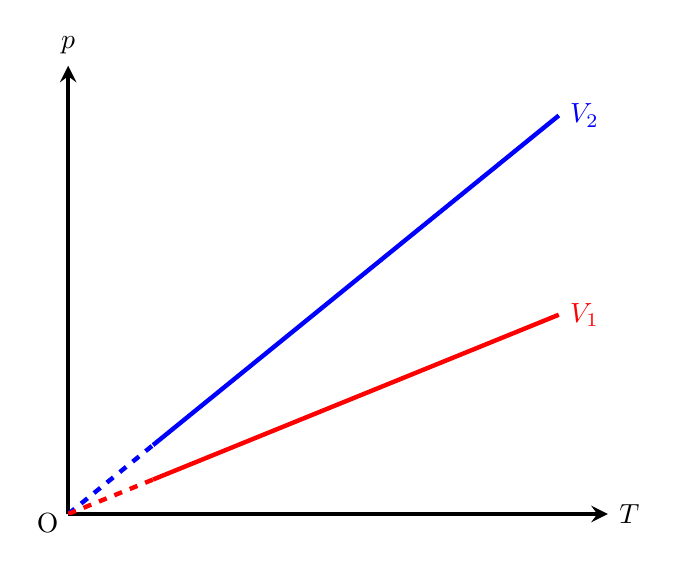
\begin{tikzpicture}  
		\begin{axis}[  ultra thick,
			xmin=0,  
			xmax=1100,  
			xtick=\empty,
			ytick=\empty,
			ymin=0,  
			ymax=900, 
			samples=300,
			xticklabels=\empty,
			yticklabels=\empty,
			axis lines=center, 
			xlabel=$T$, 
			ylabel=$p$, 
			every axis y label/.style={at=(current axis.above origin),anchor=south},  
			every axis x label/.style={at=(current axis.right of origin),anchor=west},  ]
			\addplot [ultra thick, blue, smooth,dashed, domain=0:173] {0.8*x}; 
			\addplot [ultra thick, blue, smooth, domain=173:1000] {0.8*x} node[right]{$V_2$}; 
			\addplot [ultra thick, red, smooth,dashed, domain=0:173] {0.4*x}; 
			\addplot [ultra thick, red, smooth, domain=173:1000] {0.4*x} node[right]{$V_1$};
		\end{axis}  
		\node[label={[below left]90:O}] at (0,0){};
	\end{tikzpicture}
	\captionof{figure}{Các đường đẳng tích của một khối khí lí tưởng ứng với các thể tích $V_1$ và $V_2 \left(V_2<V_1\right)$.}
\end{center}
\section{Mục tiêu bài học - Ví dụ minh hoạ}
\begin{dang}{Sử dụng định luật Boyle và định luật Charles rút ra được phương trình trạng thái của khí lí tưởng}
	\viduii{2}
{Xét một khối khí lí tưởng xác định biến đổi từ trạng thái 1 $\left(p_1, V_1, T_1\right)$ sang trạng thái 2 $\left(p_2, V_2, T_2\right)$ thông qua trạng thái trung gian 1' $\left(p_2, V', T_1\right)$.
	\begin{center}
		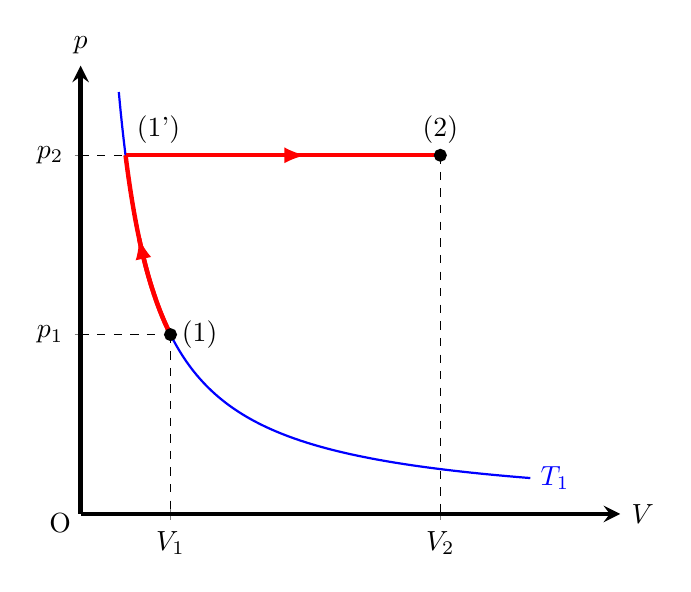
\begin{tikzpicture}  
			\begin{axis}[  ultra thick,
				xmin=0,  
				xmax=12,  
				ytick={3,6},
				xtick={2,8},
				ymin=0,  
				ymax=7.5, 
				samples=300,
				yticklabels={$p_1$, $p_2$},
				xticklabels={$V_1$, $V_2$},
				axis lines=center, 
				xlabel=$V$, 
				ylabel=$p$, 
				every axis y label/.style={at=(current axis.above origin),anchor=south},  
				every axis x label/.style={at=(current axis.right of origin),anchor=west},  ]
				\draw[line width=0.5pt, dashed] (axis cs: 0, 6) -- (axis cs: 8, 6);
				\draw[line width=0.5pt, dashed] (axis cs: 8, 6) -- (axis cs: 8, 0);
				\draw[line width=0.5pt, dashed] (axis cs: 0, 3) -- (axis cs: 2, 3);
				\draw[line width=0.5pt, dashed] (axis cs: 2, 3) -- (axis cs: 2, 0);
				\addplot [thick, blue, smooth, domain=0.85:10] {6/x} node[right] {$T_1$};  
				\addplot [ultra thick, red, smooth, domain=1:2] {6/x} ; 
				\addplot [ultra thick,-latex, red, smooth, domain=2:1.3] {6/x} ; 
				\addplot [ultra thick, red, smooth, domain=1:8] {6}; 
				\addplot [ultra thick,-latex, red, smooth, domain=1:5] {6};
				\filldraw[black] (axis cs:2,3) circle (1.5pt) node[right] {(1)};
				\filldraw[black] (axis cs:8,6) circle (1.5pt) node[above] {(2)};
				\node[above right] at (axis cs:1,6) {(1')};
			\end{axis}  
			\node[label={[below left]90:O}] at (0,0){};
		\end{tikzpicture}
		\captionof{figure}{Sơ đồ quá trình biến đổi trạng thái $(1)\rightarrow(1')\rightarrow(2)$.}
	\end{center}
	\begin{enumerate}[label=\alph*)]
		\item Chứng minh rằng $\dfrac{p_1V_1}{T_1}=\dfrac{p_2V_2}{T_2}$. Từ đó suy ra $\dfrac{pV}{T}=C$ với $C$ là hằng số phụ thuộc vào số mol khí.
		\item Xác định giá trị của $C$ theo số mol $ n$.
	\end{enumerate}
}
{\hide{
		\begin{enumerate}[label=\alph*)]
		\item Xét quá trình biến đổi trạng thái của khối khí trong từng giai đoạn:\\
		\textbf{* Quá trình biến đổi trạng thái $(1)\rightarrow(1')$:}
		\begin{center}
			\begin{tabular}{C{4cm} C{1.5cm} C{5cm}}
				\colorbox{yellow}{\textcolor{red}{\textbf{Trạng thái 1}}} & $\xrightarrow[]{T=const}$ & \colorbox{yellow}{\textcolor{red}{\textbf{Trạng thái 1'}}}\\
				$V_1$ & &$V_1'$\\
				$p_1$ & & $p_1'=p_2$
			\end{tabular}
		\end{center}
		Theo định luật Boyle:
		\begin{equation}
			\label{eq:12.1}
			p_1V_1=p_1'V_1'\Leftrightarrow p_1V_1=p_2V_1'
		\end{equation}
		\textbf{* Quá trình biến đổi $(1')\rightarrow(2)$:}
		\begin{center}
			\begin{tabular}{C{4cm} C{1.5cm} C{5cm}}
				\colorbox{green!40!white}{\textcolor{red}{\textbf{Trạng thái 1'}}} & $\xrightarrow[]{p=const}$ & \colorbox{green!40!white}{\textcolor{red}{\textbf{Trạng thái 2}}}\\
				$V_1'$ & &$V_2$\\
				$T_1'=T_1$ & & $T_2$
			\end{tabular}
		\end{center}
		Theo định luật Charles:
		\begin{equation}
			\label{eq:12.2}
			\dfrac{V_1'}{T_1'}=\dfrac{V_2}{T_2}\Rightarrow V_1'=\dfrac{V_2T_1}{T_2}
		\end{equation}
		Thay phương trình (\ref{eq:12.1}) vào phương trình (\ref{eq:12.2}):
		$$p_1V_1=\dfrac{p_2V_2T_1}{T_2}\Rightarrow \dfrac{p_1V_1}{T_1}=\dfrac{p_2V_2}{T_2}$$
		hay
		\begin{equation}
			\label{eq:12.3}
			\dfrac{pV}{T}=C\quad(\text{đpcm}).
		\end{equation}
		\item Xét trong điều kiện tiêu chuẩn $p=\SI{1}{atm}=\SI{1.013E5}{\pascal}$; nhiệt độ $T=\SI{273}{\kelvin}$ và thể tích của $\xsi{ n}{\left(\mole\right)}$ khí $V=\xsi{22,4 n}{\left(\text{lít}\right)}=\xsi{0,0224 n}{\meter^3}$.\\
		Thay vào (\ref{eq:12.3}):
		$$C=\dfrac{pV}{T}=\dfrac{\left(\SI{1.013E5}{\pascal}\right)\cdot\left(\SI{0.0224}{\meter^3}\right)\cdot n}{\SI{273}{\kelvin}}\approx\xsi{8,31 n}{\left(\dfrac{\joule}{\mole\cdot\kelvin}\right)}.$$
	\end{enumerate}
}}
	
\end{dang}
\begin{dang}{Vận dụng được phương trình trạng thái của khí lí tưởng}
	\viduii{2}{
		Trong cylanh của một động cơ đốt trong có $\SI{0.5}{\text{lít}}$ hỗn hợp khí ở áp suất $\SI{1}{atm}$ và nhiệt độ $\SI{47}{\celsius}$. Ấn piston xuống làm cho thể tích của hỗn hợp khí chỉ còn $\SI{0.05}{\text{lít}}$ và áp suất tăng lên $\SI{15}{atm}$. Giả thiết rằng hỗn hợp khí tăng tuân theo phương trình trạng thái của khí lí tưởng. Tính nhiệt độ của hỗn hợp khí ở trạng thái nén.
	}
	{\hide{
		\begin{center}
			\begin{tabular}{C{4cm} C{1.5cm} C{5cm}}
				\colorbox{green!40!white}{\textcolor{red}{\textbf{Trạng thái đầu}}} & $\xrightarrow[]{ n=const}$ & \colorbox{green!40!white}{\textcolor{red}{\textbf{Trạng thái sau}}}\\
				$p_1=\SI{1}{atm}$ & & $p_2=\SI{15}{atm}$\\
				$V_1=\SI{0.5}{\text{lít}}$ & &$V_2=\SI{0.05}{\text{lít}}$\\
				$T_1=\SI{320}{\kelvin}$ & & $T_2=?$
			\end{tabular}
		\end{center}
		Do lượng khí là không đổi, áp dụng phương trình trạng thái của khí lí tưởng:
		$$\dfrac{p_1V_1}{T_1}=\dfrac{p_2V_2}{T_2}$$
		$$\Rightarrow T_2=\dfrac{p_2V_2}{p_1V_1}\cdot T_1=\dfrac{\left(\SI{15}{atm}\right)\cdot\left(\SI{0.05}{\text{lít}}\right)}{\left(\SI{1}{atm}\right)\cdot\left(\SI{0.5}{\text{lít}}\right)}\cdot\left(\SI{320}{\kelvin}\right)=\SI{480}{\kelvin}.$$
	}}
	
	\viduii{3}
	{Tăng đồng thời nhiệt độ của một khối khí lí tưởng từ $\SI{27}{\celsius}$ lên $\SI{177}{\celsius}$ và áp suất từ $\SI{100}{\kilo\pascal}$ lên $\SI{300}{\kilo\pascal}$. Hỏi khối lượng riêng của khối khí tăng hay giảm bao nhiêu lần?
		
	}
	{\hide{
			\begin{center}
			\begin{tabular}{C{4cm} C{1.5cm} C{5cm}}
				\colorbox{green!40!white}{\textcolor{red}{\textbf{Trạng thái đầu}}} & $\xrightarrow[]{ n=const}$ & \colorbox{green!40!white}{\textcolor{red}{\textbf{Trạng thái sau}}}\\
				$p_1=\SI{100}{\kilo\pascal}$ & & $p_2=\SI{300}{\kilo\pascal}$\\
				$T_1=\SI{300}{\kelvin}$ & & $T_2=\SI{450}{\kelvin}$\\
				$\rho_1, V_1$ & & $\rho_2, V_2$
			\end{tabular}
		\end{center}
		Gọi $\rho_1$, $V_1$ và $\rho_2$, $V_2$ lần lượt là khối lượng riêng, thể tích lúc đầu và lúc sau của khối khí đang xét; $m$ là khối lượng của khối khí.\\
		Áp dụng phương trình trạng thái của khí lí tưởng:
		$$pV=\dfrac{m}{\mu}RT\Rightarrow \rho=\dfrac{m}{V}=\dfrac{p\mu}{RT}.$$
		Như vậy:
		$$\dfrac{\rho_2}{\rho_1}=\dfrac{p_2}{p_1}\cdot\dfrac{T_1}{T_2}=\dfrac{\SI{300}{\kilo\pascal}}{\SI{100}{\kilo\pascal}}\cdot\dfrac{\SI{300}{\kelvin}}{\SI{450}{\kelvin}}=2.$$
		Như vậy, khối lượng riêng của khối khí lí tưởng này tăng 2 lần.
	}}
	
	\viduii{3}
	{ \begin{minipage}{0.7\textwidth}
			Một cylanh đặt thẳng đứng có tiết diện là $S=\SI{100}{\centi\meter^2}$, chứa không khí ở nhiệt độ $t_1=\SI{27}{\celsius}$. Ban đầu cylanh được đậy bằng một piston cách đáy $h=\SI{50}{\centi\meter}$. Piston có thể trượt không ma sát dọc theo mặt trong cylanh. Đặt lên trên piston một quả cân có trọng lượng $P=\SI{500}{\newton}$. Piston dịch chuyển xuống đoạn $\ell=\SI{10}{\centi\meter}$ rồi dừng lại.\\
			Tính nhiệt độ của khí trong cylanh sau khi piston dừng lại. Biết áp suất khí quyển là $p_0=\SI{E5}{\newton/\meter^2}$. Bỏ qua khối lượng của piston.
		\end{minipage}
		\begin{minipage}{0.3\textwidth}
			\begin{center}
				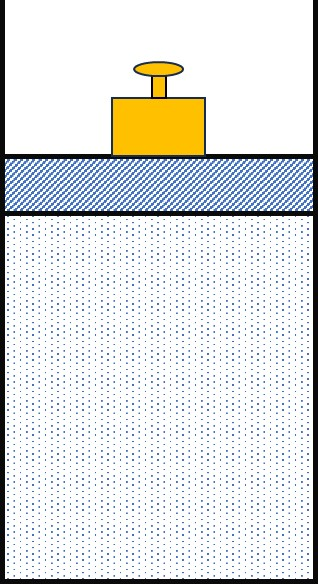
\includegraphics[width=0.35\linewidth]{../figs/VN12-Y24-PH-SYL-012-1}
			\end{center}
		\end{minipage}
	}
	{\hide{
		Ban đầu khi piston cân bằng, áp lực do khí quyển tác dụng lên piston bằng áp lực do khí trong bình tác dụng:
		$$p_1=p_0=\SI{E5}{\pascal}.$$
		Khi đặt quả cân lên piston và piston lại cân bằng, áp lực của khí trong cylanh tác dụng lên piston bằng áp lực khí quyển và trọng lực của quả cân:
		$$p_2=p_0+\dfrac{P}{S}=\SI{E5}{\pascal}+\dfrac{\SI{500}{\newton}}{\SI{100E-4}{\meter^2}}=\SI{1.5E5}{\pascal}.$$
		\begin{center}
			\begin{tabular}{C{4cm} C{1.5cm} C{5cm}}
				\colorbox{green!40!white}{\textcolor{red}{\textbf{Trạng thái đầu}}} & $\xrightarrow[]{ n=const}$ & \colorbox{green!40!white}{\textcolor{red}{\textbf{Trạng thái sau}}}\\
				$p_1=\SI{E5}{\pascal}$ & & $p_2=\SI{1.5E5}{\pascal}$\\
				$V_1=Sh$ & & $V_2=S\left(h-\ell\right)$\\
				$T_1=\SI{300}{\kelvin}$ & & $T_2=?$
			\end{tabular}
		\end{center}
		Áp dụng phương trình trạng thái của khí lí tưởng:
		$$\dfrac{p_1V_1}{T_1}=\dfrac{p_2V_2}{T_2}$$
		$$\Rightarrow T_2=\dfrac{p_2}{p_1}\cdot\dfrac{V_2}{V_1}\cdot T_1=\dfrac{p_2}{p_1}\cdot\dfrac{\left(h-\ell\right)}{h}\cdot T_1$$
		$$\Leftrightarrow T_2=\dfrac{\SI{1.5E5}{\pascal}}{\SI{E5}{\pascal}}\cdot\left(\dfrac{\SI{50}{\centi\meter}-\SI{10}{\centi\meter}}{\SI{50}{\centi\meter}}\right)\cdot\left(\SI{300}{\kelvin}\right)=\SI{360}{\kelvin}.$$
	}}
	
\end{dang}
\begin{dang}{Vận dụng được định luật Dalton \textit{(mở rộng)}}
	\ppgiai{Ở một nhiệt độ và thể tích xác định, áp suất toàn phần của một hỗn hợp khí gồm các khí không phản ứng hoá học với nhau bằng tổng áp suất riêng phần của mỗi khí thành phần có trong hỗn hợp:
		\begin{equation}
			p=p_1+p_2+\dots+p_n=\sum_{1}^{n}p_i
	\end{equation}}
	\viduii{4}
	{Bình A có dung tích $V_1=\SI{3}{\text{lít}}$, chứa một chất khí ở áp suất $p_1=\SI{2}{at}$. Bình B dung tích $V_2=\SI{4}{\text{lít}}$, chứa một chất khí ở áp suất $p_2=\SI{1}{at}$. Nhiệt độ trong hai bình là như nhau. Nối hai bình A, B thông với nhau bằng một ống dẫn nhỏ. Biết không có phản ứng hoá học xảy ra giữa hai khí trong các bình. Tính áp suất của hỗn hợp khí.
		
	}
	{\hide{Gọi áp suất riêng phần của mỗi khí trong hỗn hợp khi hai bình thông với nhau là $p_1'$ và $p_2'$.\\
		Trong quá trình nối hai bình với nhau, nhiệt độ của khí trong hai bình không đổi.\\
		\textbf{* Xét quá trình biến đổi trạng thái của khí trong bình A}
		\begin{center}
			\begin{tabular}{C{4cm} C{1.5cm} C{5cm}}
				\colorbox{yellow}{\textcolor{red}{\textbf{Trạng thái 1}}} & $\xrightarrow[]{T=const}$ & \colorbox{yellow}{\textcolor{red}{\textbf{Trạng thái 1'}}}\\
				$V_1=\SI{3}{\text{lít}}$ & &$V_1'=V_1+V_2=\SI{7}{\text{lít}}$\\
				$p_1=\SI{2}{at}$ & & $p_1'=?$
			\end{tabular}
		\end{center}
		Theo định luật Boyle:
		$$p_1V_1=p_1'V_1'\Rightarrow p_1'=\dfrac{p_1V_1}{V_1'}=\dfrac{\left(\SI{2}{at}\right)\cdot\left(\SI{3}{\text{lít}}\right)}{\SI{7}{\text{lít}}}=\xsi{\dfrac{6}{7}}{at}.$$
		\textbf{* Xét quá trình biến đổi trạng thái của khí trong bình B}
		\begin{center}
			\begin{tabular}{C{4cm} C{1.5cm} C{5cm}}
				\colorbox{green!40!white}{\textcolor{red}{\textbf{Trạng thái 2}}} & $\xrightarrow[]{T=const}$ & \colorbox{green!40!white}{\textcolor{red}{\textbf{Trạng thái 2'}}}\\
				$V_2=\SI{4}{\text{lít}}$ & &$V_2'=V_1+V_2=\SI{7}{\text{lít}}$\\
				$p_2=\SI{1}{at}$ & & $p_2'=?$
			\end{tabular}
		\end{center}
		Theo định luật Boyle:
		$$p_2V_2=p_2'V_2'\Rightarrow p_2'=\dfrac{p_2V_2}{V_2'}=\dfrac{\left(\SI{1}{at}\right)\cdot\left(\SI{4}{\text{lít}}\right)}{\SI{7}{\text{lít}}}=\xsi{\dfrac{4}{7}}{at}.$$
		Áp dụng định luật Dalton, áp suất của hỗn hợp khí:
		$$p'=p_1'+p_2'=\xsi{\dfrac{10}{7}}{at}\approx\SI{1.43}{at}.$$
	}}
\end{dang}

